\documentclass[10pt,a4paper]{article}
\usepackage[margin=1.8cm]{geometry}
\usepackage{amsmath,amssymb}
\usepackage{booktabs}
\usepackage{graphicx}
\usepackage[T1]{fontenc}
\usepackage{microtype}
\usepackage[colorlinks,linkcolor=black,citecolor=black,urlcolor=blue]{hyperref}
\usepackage{xcolor}
\usepackage{tabularx}
% A GATE THAT PASSED IS GREEN AND A GATE THAT FAILED IS RED, in the table and nowhere else -- the
% colour is the verdict, so it is never spent on decoration.
\definecolor{gpass}{HTML}{1B7F4B}
\definecolor{gfail}{HTML}{B03A2E}
\newcommand{\pass}[1]{\textcolor{gpass}{\textbf{#1}}}
\newcommand{\fail}[1]{\textcolor{gfail}{\textbf{#1}}}
\newcolumntype{L}{>{\raggedright\arraybackslash}X}
\usepackage{titlesec}
\titlespacing*{\section}{0pt}{6pt}{2pt}
\newcommand{\code}[1]{\texttt{#1}}
\newcommand{\op}[1]{\texttt{#1}}
\title{\vspace{-1.4cm}\textbf{The cell--cell junction:\\
\normalsize myosin as a density on a belt, through a division}}
\author{}
\date{\vspace{-0.9cm}\small \texttt{prototype/ecm/junction\_ops.py} $\cdot$
\texttt{medioapical\_ops.py} $\cdot$
\texttt{test\_01\{,b,c\}*.py} $\cdot$
\texttt{log/okuda\_ECM/01, 01b, 01c} $\cdot$ 10 August 2026}
\setlength{\parindent}{0pt}\setlength{\parskip}{0.55em}
\begin{document}\maketitle\vspace{-1.0cm}

\section*{1.\; Mechanism}

In a vertex model every cell--cell contact pulls with the same strength. Real contractility is not
uniform: myosin accumulates on some junctions and not others, and where it accumulates the junction
pulls harder and shortens, which is how cells exchange neighbours.

\textbf{A junction is a surface, and it enters the energy as a line.} The lateral interface between
two cells is of order $\ell\times h$, $\ell$ its apical extent and $h$ the cell's height. This
epithelium is one triangulated shell --- a cell is a face and its ``volume'' is the wedge from the
tissue centre --- so there is no $h$, and the junction enters as a line of length $\ell_e$ with the
third dimension absorbed into the line tension $\Lambda$. That is the right geometry for the term it
multiplies rather than a compromise: the contractile actomyosin of an adherens junction is a
\emph{belt} at the apical rim of that interface, a cable of length $\ell_e$; what is spread over the
lateral \emph{area} is cadherin adhesion, which this energy does not carry.

\textbf{The consequence is what the symbol means.} $\Lambda\sum_e m_e\ell_e$ is a tension times a
length, so $m_e$ is a \textbf{density} --- myosin per unit length of belt --- and the \emph{amount} on
a junction is $N_e=m_e\ell_e$. Everything below follows from that identification, and the model's own
inheritance rule is only correct if it is true: when \op{divide\_3d} cuts a contact $(a,b)$ into
$(a,n)$ and $(n,b)$, \emph{nothing physical has happened} --- the same two cells still touch across the
same interface --- and copying the parent's $m$ onto both halves conserves the amount only because $m$
is intensive. Had $m$ been an amount, the identical line of code would have doubled the tissue's
myosin at every division and nothing would have failed.

\textbf{Two pools, because the biology has two.} An epithelial cell carries a \textbf{medioapical}
meshwork spread over its apical face and a \textbf{junctional} belt at the rim, coupled by outward
flow, and germband extension uses both \cite{munjal2015}. The first is areal, the second linear. So
``should myosin scale with area or with length'' has the answer \emph{both}, and the repair for the
defect above is not a better drive but a conserved amount with a derived density. In a dividing cell,
almost all of the myosin goes to the \textbf{cytokinetic ring}, which constricts exactly at the nascent
interface; in epithelia the new adherens junction is built out of it, with the neighbouring cell
contributing \cite{herszterg2013,founounou2013}.

\begin{figure}[t]\centering
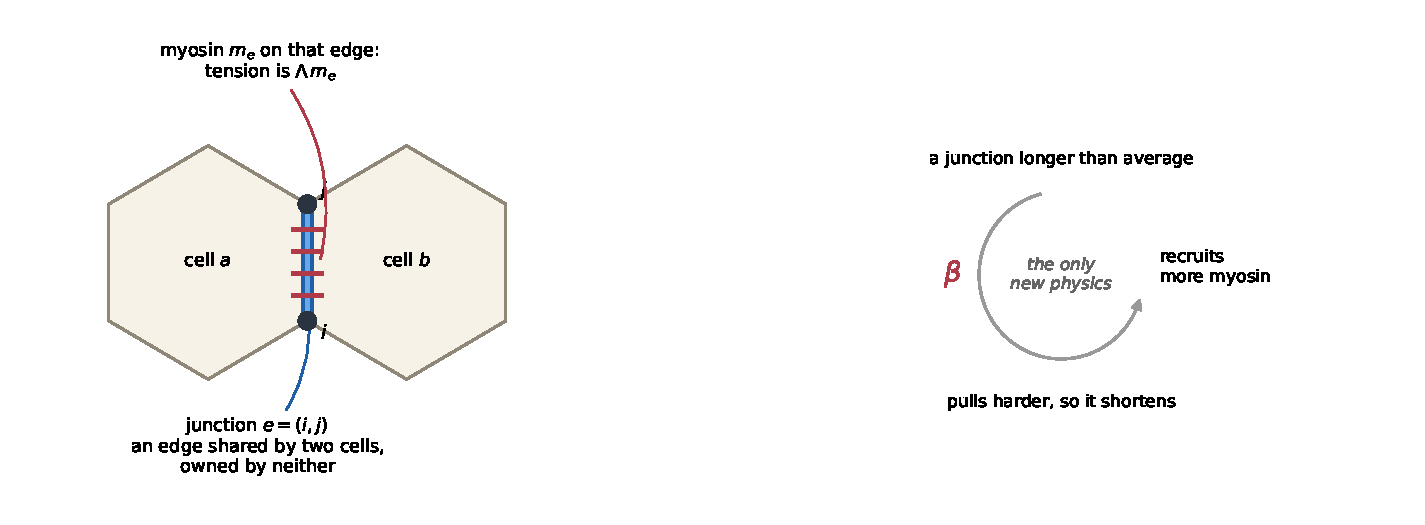
\includegraphics[width=\textwidth]{fig_junction_schematic.pdf}
\caption{Two cells share an edge, and that edge \emph{is} the junction --- it belongs to neither, which
is why its state is keyed by the pair of vertices rather than stored on a cell. Myosin sits on the
shared edge and multiplies its tension. Right: the feedback, which is the only thing here the original
model cannot already do.}
\end{figure}

\section*{2.\; Equations and symbols}

\textbf{The energy the myosin multiplies}, unchanged from the stock 3D vertex model except for $m_e$:
%
\begin{equation}
E=\sum_f\Bigl[K_A(A_f-A^0_f)^2+K_P(P_f-P^0_f)^2+\tfrac12\Gamma P_f^2+K_V(v_f-v^0_f)^2\Bigr]
 +\Lambda\!\sum_e m_e\ell_e+K_R\sum_i(|\mathbf x_i|-R_0)^2 .
\label{eq:avm}
\end{equation}
%
With $m_e\equiv1$ this is the stock Okuda energy \cite{okuda2013,okuda2018} and every prior run is
bit-identical.

\textbf{The two pools.} $\rho_f$ is areal and lives on the cell; $n_e$ is linear and lives on the
junction; the flux between them is per unit length of belt, because there is $\ell_e$ of belt to
receive it:
%
\begin{align}
M_f&=\rho_fA_f, &\frac{\mathrm dM_f}{\mathrm dt}
 &=k_{\rm on}A_f-\frac{M_f}{\tau_{\rm med}}-\!\!\sum_{e\in\partial f}\!\!J_{f\to e},
 &J_{f\to e}&=k_{\rm ex}\rho_f\ell_e\bigl(1+\beta_T(T_e/\langle T\rangle-1)\bigr),
\label{eq:med}\\[2pt]
N_e&=n_e\ell_e, &\frac{\mathrm dN_e}{\mathrm dt}
 &=\sum_{f\ni e}J_{f\to e}-\frac{N_e}{\tau_{\rm jun}},
 &m_e&=a\,n_e/\langle n\rangle .
\label{eq:jun}
\end{align}
%
\textbf{The setpoint is now intensive}, which is the whole point: the belt's supply is per unit length,
so
%
\begin{equation}
n^\ast_e=\tau_{\rm jun}k_{\rm ex}(\rho_f+\rho_g)
\label{eq:nstar}
\end{equation}
%
--- two-sided, because a junction is fed by both cells it separates --- carries no $\ell_e$, and half a
junction relaxes toward what the whole junction was relaxing toward. The one-pool law does not: its
target is $m^{ss}_e=a\ell_e/\langle\ell\rangle$, and $\ell_e$ is extensive, so a cut halves it.

\begin{center}\itshape the drive of a feedback must be intensive.\end{center}

Tension is (cutting a cable in two does not halve the tension in it); strain and strain rate are;
length is not.

\textbf{The cytokinetic ring} seeds every interface with \emph{both} endpoints new --- exactly the case
the inheritance rule excludes --- and \emph{debits} the two daughters' cortical pools, so it moves
myosin instead of creating it:
%
\begin{equation}
n_e=\texttt{ring}\times n^\ast,\qquad
\rho_{f,g}\ \text{reduced by the same amount}.
\label{eq:ring}
\end{equation}

\textbf{One prediction arrives unbidden.} The steady state of Eq.~\eqref{eq:med} is
$\rho^\ast=k_{\rm on}/(1/\tau_{\rm med}+k_{\rm ex}P_f/A_f)$: a cell with more perimeter per unit area
drains faster and holds less medioapical myosin. $P_f/A_f$ is fixed by shape alone, so the model says
--- with nothing added to make it say so --- that as a tissue divides into smaller cells, myosin shifts
off the cortex and onto the belts. That is gate J8.

\smallskip
{\small\begin{tabular}{@{}llp{8.6cm}@{}}\toprule
symbol & is & of what\\\midrule
$m_e$ & myosin on junction $e$ & a DENSITY, dimensionless multiplier on $\Lambda$, mean $1$\\
$n_e$, $N_e$ & line density, amount & $N_e=n_e\ell_e$; what is stored is $n_e$\\
$\rho_f$, $M_f$ & areal density, amount & $M_f=\rho_fA_f$, on the cell's apical face\\
$k_{\rm on}$ & assembly rate & myosin assembled per unit \emph{apical area} per frame\\
$k_{\rm ex}$ & export rate & drawn from the cortex per unit \emph{length} of belt per frame\\
$\tau_{\rm med},\tau_{\rm jun}$ & turnover times & in FRAMES; see the caveat at the end of \S4\\
$\beta_T$ & tension bias on the flux & $0$ in the reported run: pure transport, deliberately\\
\texttt{ring} & the ring's deposit & in units of $n^\ast$, so it cannot drift with the tissue's mean\\
$a$ & global activity & multiplies every junction equally\\
$\Lambda,\Gamma,K_P$ & line tension, contractility, perimeter stiffness & read OFF
  \op{shape\_energy\_3d}, not restated --- a tension computed from different constants is the tension
  of a different tissue\\
\bottomrule\end{tabular}}

\section*{3.\; The Plexus2 container}

\textbf{One structural claim.} A junction is a \emph{relation between two vertices}, not a body: it
belongs to neither cell, so its state is keyed by the vertex pair and not stored on a face. That is
what makes the inheritance rules local and what makes the sync operator below possible at all.

\begin{center}\small
\begin{tabular}{@{}llll@{}}\toprule
\textbf{set} & \textbf{kind} & \textbf{one element is} & \textbf{state it carries}\\\midrule
\code{cell}    & node, depth 1 & one epithelial cell & $A,P,V$ and their targets, age, \code{ndiv},
  $\rho_f$\\
\code{vertex}  & node, depth 1 & a corner of the apical mesh & \code{pos}\\
\code{junction}& \textbf{edge} $\subseteq$ \code{vertex}$^2$ & a cell--cell contact & $n_e$, $\ell_e$,
  $m_e$ (written to \code{m["myo"]})\\
\bottomrule\end{tabular}
\end{center}

\begin{center}\footnotesize
\begin{tabular}{@{}lllp{4.4cm}p{3.1cm}@{}}\toprule
\textbf{operator} & \textbf{kind} & \textbf{acts on} & \textbf{mechanism} & \textbf{its gate}\\\midrule
\op{medioapical\_myosin} & Lateral & \code{cell} & Eq.~\eqref{eq:med}; emits $J_{f\to e}$ & J8\\
\op{junction\_myosin} \code{[two\_pool]} & \textbf{Structural} & \code{junction} &
  Eq.~\eqref{eq:jun}; integrates $N_e$, writes $m_e$ & J1--J4\\
\op{cytokinetic\_ring}   & Structural & \code{junction} & Eq.~\eqref{eq:ring}; seeds newborns, debits
  the daughters & J5--J7\\
\op{junction\_myosin\_sync} & \textbf{Rewire} & \code{junction} & re-keys $m_e,N_e$ by vertex pair
  after the topology operators & J9\\
\op{reconnect\_t1\_3d}, \op{divide\_3d} & Rewire, Divide & \code{junction}, \code{cell} & neighbour
  exchange and cytokinesis \cite{okuda2013} & J10\\
\bottomrule\end{tabular}
\end{center}

\textbf{Three placements carry the argument.} \code{two\_pool} is registered as a \code{model=} of the
existing contract and not an \code{implementation=}: its parameters $\{\tau_{\rm jun},a\}$ are disjoint
from the default's $\{a,\tau,\beta,\code{keyed\_on}\}$, so there is no common operating point at which
to call them two ways of computing one thing --- per plexus2, swapping a model \emph{is} an
experiment. They share the contract's kind and write the same channel, so \op{shape\_energy\_3d} cannot
tell them apart and the comparison is fair. The medioapical operator is scheduled \emph{before} the
belt's, so a frame's flux is the flux that frame's cells produced. And the sync runs \emph{after} the
topology operators:

\smallskip
{\footnotesize
\begin{verbatim}
  ... -> medioapical_myosin -> junction_myosin -> cell_mechanics
      -> edge_flip -> cell_divide -> cytokinetic_ring -> junction_sync -> ...
\end{verbatim}}
\smallskip

\textbf{The sync operator is why any of this is measurable.} \op{junction\_myosin} writes
\code{m["myo"]} sized to the half-edge buffer at its own slot; \op{reconnect\_t1\_3d} rewires those
arrays and \op{divide\_3d} lengthens them later in the same frame, and \op{topo\_snapshot\_3d} then
recorded the frame's edges beside the \emph{previous} topology's myosin. Every division frame --- which
is precisely where this note's measurement lives --- was one of the broken ones (J9).

\section*{4.\; Gates}

A gate is a number with a threshold decided \emph{before} the run and a stated consequence if it
fails. Two builds of the same $401$-frame tissue differ only in the myosin model, and within each,
junctions a division \emph{cut} are compared against \emph{intact} ones over the same interval. The
control is not optional: two frames of ordinary dynamics move an untouched junction too, and without it
every division looks like a leak.

\smallskip
{\scriptsize\setlength{\tabcolsep}{4pt}
\begin{tabularx}{\textwidth}{@{}llLl@{}}\toprule
& \textbf{gate} & \textbf{threshold} & \textbf{measured}\\\midrule
\multicolumn{4}{@{}l}{\textit{the amount survives a re-meshing} (\op{01b}, $13{,}083$ / $12{,}320$ cuts)}\\
J1 & $(N_1{+}N_2)/N_{\rm parent}$ over $(\ell_1{+}\ell_2)/\ell_{\rm parent}$, cut &
     $\le$ the intact control & one-pool $1.0068$, two-pool \pass{1.0043}\\
J2 & the same ratio on intact junctions (the control) & --- & $1.0092$ / $1.0093$\\
J3 & setpoint of a half over its parent's & $=1$; length-keyed gives $\tfrac12$ &
     one-pool \fail{0.514}, by design\\
J4 & $m$ twenty frames after the cut, over intact & $>0.90$ & one-pool \fail{0.797}, two-pool
     \pass{0.939}\\
\multicolumn{4}{@{}l}{\textit{the newborn junction} (\op{01c})}\\
J5 & daughter--daughter interface, $m/\langle m\rangle$ at birth & within $0.10$ of $1$ &
     absolute \fail{0.628}; ring$=1$ \pass{0.920}; ring$=3$ $2.483$\\
J6 & drift of that value across the run & $<0.15$ & absolute \fail{0.33}; ring$=1$ \pass{0.12}\\
J7 & the deposit relaxes on the belt's own timescale & $e$-fold within $20\%$ of $\tau_{\rm jun}=20$ &
     \pass{$\sim$19} frames ($2.48\to1.22$ over $30$)\\
\multicolumn{4}{@{}l}{\textit{the prediction nothing was added to make} (\op{01b})}\\
J8 & medioapical share falls as $\langle P_f/A_f\rangle$ rises & monotone, both &
     share $0.214\to$ \pass{0.096}, $P/A$ $3.38\to$ \pass{5.19}\\
\multicolumn{4}{@{}l}{\textit{the bookkeeping} (\op{01}, the nominal)}\\
J9 & myosin array length equals the edge array's & $0$ of $200$ short & \fail{56} before the sync
     (by $6$--$1356$); \pass{0} after\\
J10& the sync perturbs nothing: positions, divisions, T1s & bit-identical & \pass{bit-identical}\\
J11& T1 per cell per frame: does the law change the observable & any separation &
     $0.00221$ vs \pass{0.00373} ($1.69\times$)\\
\multicolumn{4}{@{}l}{\textit{the scale the note is quoted in} (\op{0u\_units})}\\
U1& one frame, from 4.93 doublings at a 12--24\,h cycle & $[8.8, 17.7]$ min & \pass{10 min}\\
U2& $\tau_{\rm jun}=20$ frames --- maturation, NOT myosin turnover ($1$--$2$ min) & $[30, 600]$ min & \pass{200 min}\\
U3& cell diameter (the length CALIBRATION) & $[5, 15]$ um & \pass{8.5 um}\\
U4& junction length at the last frame & $[2, 15]$ um & \pass{4.6 um}\\
U5& time between neighbour exchanges, per cell & $[20, 200]$ h & \pass{44.68 h}\\
\bottomrule\end{tabularx}}
\smallskip


\textbf{The run declares its scale, and these numbers are what it makes of it.} Three base scales
under \code{general.units:} and everything else derived (\code{plexus/units.py}): $1$ box unit
$=1172\,\mu$m, because a cell is $8.5\,\mu$m and the tissue is solved at $10\,\mu$m per tissue
unit; $1$ frame $=600$ s, because $200\to6{,}076$ cells is $4.93$ doublings and a $12$--$24$ h
cycle puts the run at $2.5$--$4.9$ days; $1$ force unit $=9162$ nN, set so the stroma's
\code{youngs: 15} is $100$ Pa --- a collagen I gel at $1$--$3$ mg/ml. Only the force scale is
\emph{chosen}, and it is chosen on the softest and best-measured body rather than on the sheet under
dispute. Without this block the loader says the run is dimensionless and no result from it may carry
a unit, which was the state of every run in this folder until now.

\textbf{Two conventions make these mean what they say.} \textbf{A cut is measured against an intact
control on the same frames}, because two frames of dynamics move an untouched junction by $0.9\%$ and
a raw ratio of $1.007$ would otherwise read as a leak. And \textbf{a newborn's value is read against
the tissue's own mean, binned by time}: \code{myo\_new} was an absolute line density in a model whose
mean line density runs $1.07\to1.97\to1.48$ over $401$ frames, so what a new junction started with was
decided by the frame index --- the run-median hides that, and J6 is the gate that does not.

\textbf{The residual in J4 is not a leftover artifact.} Writing $N_e=n_e\ell_e$ in Eq.~\eqref{eq:jun}
gives $\dot n_e=k_{\rm ex}\rho-n_e/\tau_{\rm jun}-n_e\,\mathrm d\ln\ell_e/\mathrm dt$: a junction whose
length is changing dilutes or concentrates its own belt. Freshly cut halves relax and lengthen, so they
dilute. That term is advection of a conserved species along a moving cable, which is physics; the
$20\%$ it replaces was arithmetic. The same term is why J5 sits at $0.92$ and not $1.00$ --- mature
junctions are not \emph{at} $n^\ast$, because the tissue's mean junction length falls $0.75\to0.46$ as
cells divide and a shortening belt concentrates above its own steady state.

\textbf{What the gates do not license.} The operating point: $k_{\rm on}$ was set to
$1/\tau_{\rm med}+k_{\rm ex}\langle P/A\rangle_0=0.219$ so the cortical density \emph{starts} at its own
steady state, and $\tau_{\rm med}=\tau_{\rm jun}=20$ frames with $k_{\rm ex}=0.05$ are chosen numbers.
$\beta_T=0$ in the reported run --- pure transport, deliberately, so a tension bias added later has to
beat what geometry already does (J8). There is no pulsatility, which is the mechanism the medioapical
pool is famous for: Munjal's pulses need advection-mediated positive feedback with dissociation as the
negative arm, a third state variable and an advection term. And \textbf{one frame is still not anchored
to a time}: the run's own growth fixes it at $9$--$18$ minutes per frame, at which junctional myosin
turnover ($1$--$2$ minutes) is a tenth of a frame and the belt is adiabatic. A $20$-frame memory on a
junction can legitimately be \emph{maturation} --- E-cadherin accumulation over tens of minutes to
hours --- so $\tau_{\rm jun}$ should be renamed and re-sourced rather than quoted as turnover.

\begin{figure}[h]\centering
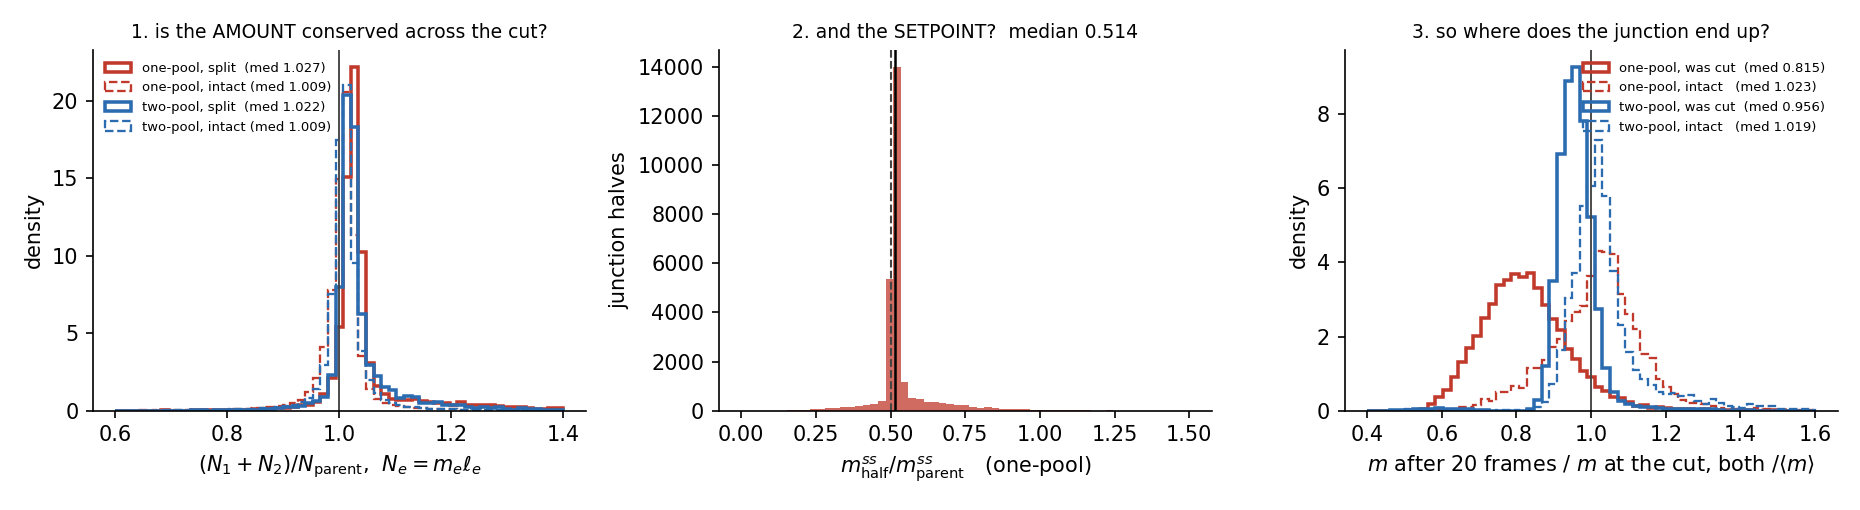
\includegraphics[width=\textwidth]{fig_junction_conservation.png}
\caption{J1--J4. Left: the amount across a cut, both models, against the intact control --- the offset
from $1$ is the $2\%$ by which the two halves are longer than the parent they replace, not a leak.
Middle: the one-pool setpoint of a half over its parent's, which is $1/2$ because the setpoint is
proportional to a length that was just halved (J3). Right: where the junction actually ends up twenty
frames later (J4).}
\end{figure}

\begin{figure}[h]\centering
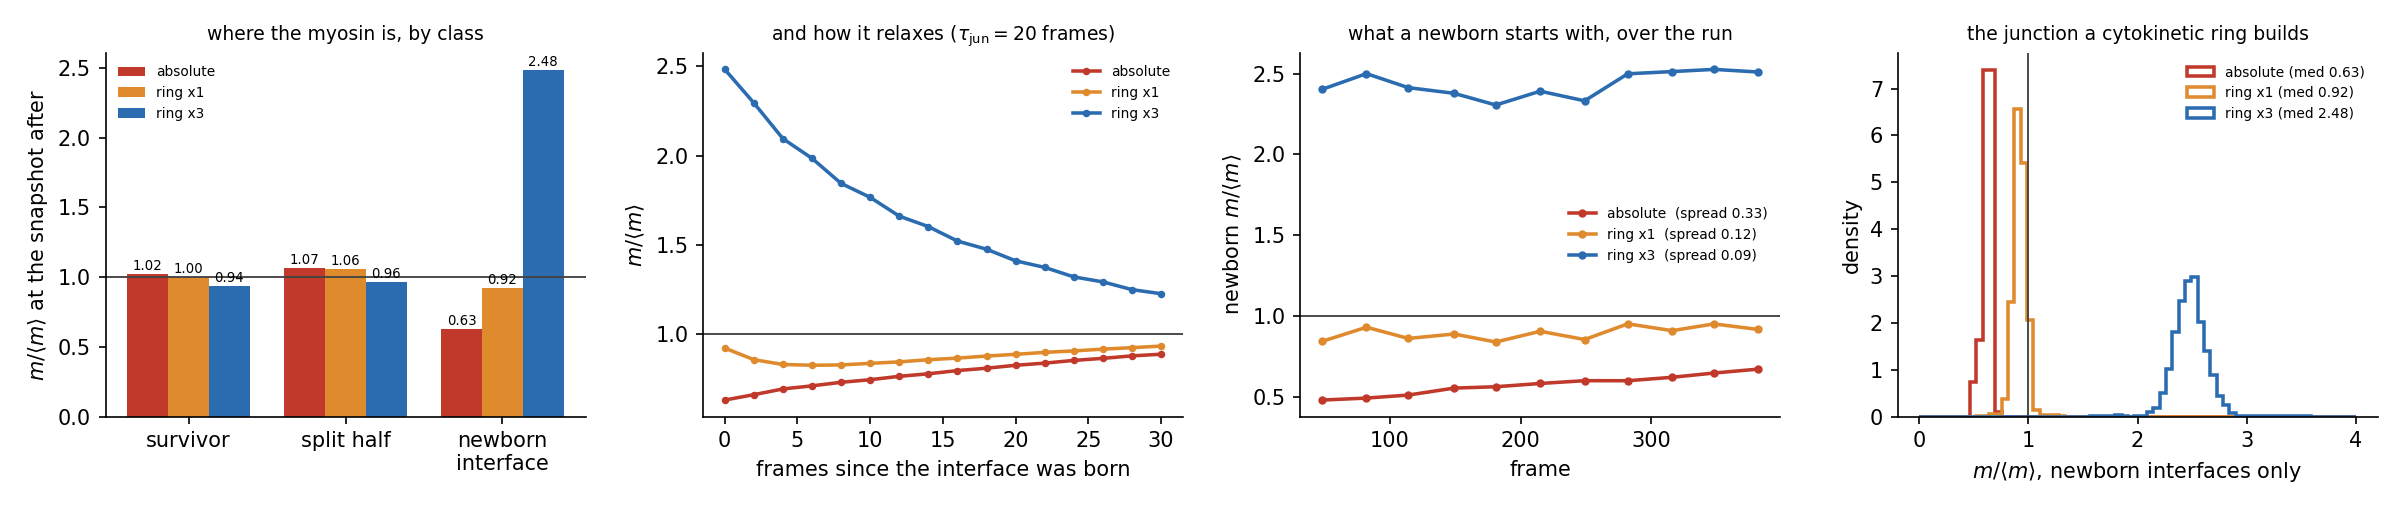
\includegraphics[width=\textwidth]{fig_junction_newborn.png}
\caption{J5--J7. Left: myosin by junction class. Middle-left: the deposit relaxing --- \texttt{ring}$=3$
falls $2.48\to1.22$ over $30$ frames toward the \texttt{ring}$=1$ level, an $e$-folding of $\sim\!19$
frames against a $\tau_{\rm jun}$ of $20$ that nobody fitted: the ring needs no timescale of its own
because the belt already has one. Middle-right: J6, what a newborn starts with, binned by frame --- the
absolute rule drifts $0.479\to0.670$, both ring runs are flat.}
\end{figure}

\section*{5.\; References}

{\small
\begin{thebibliography}{99}\setlength{\itemsep}{0pt}
\bibitem{okuda2013} Okuda, S., Inoue, Y., Eiraku, M., Sasai, Y., Adachi, T. (2013) Reversible network
reconnection model for simulating large deformation in dynamic tissue morphogenesis.
\emph{Biomech. Model. Mechanobiol.} \textbf{12}(4):627--644.
\bibitem{okuda2018} Okuda, S., Miura, T., Inoue, Y., Adachi, T., Eiraku, M. (2018) Combining Turing and
3D vertex models reproduces autonomous multicellular morphogenesis. \emph{Sci. Rep.} \textbf{8}:2386.
\bibitem{munjal2015} Munjal, A., Philippe, J.-M., Munro, E., Lecuit, T. (2015) A self-organized
biomechanical network drives shape changes during tissue morphogenesis. \emph{Nature} \textbf{524}:351--355.
\bibitem{fgonzalez2009} Fernandez-Gonzalez, R., Simoes, S.\,de\,M., R\"oper, J.-C., Eaton, S., Zallen, J.A.
(2009) Myosin II dynamics are regulated by tension in intercalating cells. \emph{Dev. Cell}
\textbf{17}(5):736--743.
\bibitem{herszterg2013} Herszterg, S., Leibfried, A., Bosveld, F., Martin, C., Bellaiche, Y. (2013)
Interplay between the dividing cell and its neighbors regulates adherens junction formation during
cytokinesis in epithelial tissue. \emph{Dev. Cell} \textbf{24}(3):256--270.
\bibitem{founounou2013} Founounou, N., Loyer, N., Le Borgne, R. (2013) Septins regulate the
contractility of the actomyosin ring to enable adherens junction remodeling during cytokinesis of
epithelial cells. \emph{Dev. Cell} \textbf{24}(3):242--255.
\end{thebibliography}}

\end{document}
